\chapter{Propiedades térmicas reticulares} \label{Ch:05}

En este Tema se estudia la parte más \textit{física} de las vibraciones atómicas en los sólidos. En concreto, veremos cómo se pueden entender desde la dinámica de red propiedades como \textit{calor específico}, la \textit{conductividad térmica} y la \textit{dilatación térmica} de los sólidos.

\section{Densidad de modos}

\subsection{Condiciones de contorno}

Se trata de incluir cuantitativamente el hecho de que todo cristal es finito. Sea un cristal de dimensiones $N_i \an_i  \ (i=1,2,3)$ siendo los $\an_i$ ejes primitivos $N=N_1N_2N_3$ el número de celdas primitivas. Imponiendo sobre las soluciones $\un(\Rn,t)= \epsilonn e^{i(\kn \cdot \Rn - \omega t)}$ las llamadas \textbf{condiciones de contorno periódicas} o \textbf{condiciones de contorno de Born-von Karman}, $\un(\Rn + N_i \an_i) = \un (\Rn)$ para cualquier $i=1,2,3$ se encuentra que los vectores $\kn$ son de la forma

\begin{eqnarray}
	\kn = \frac{n_1}{N_1} \bn_1 + \frac{n_2}{N_2} \bn_2 + \frac{n_3}{N_3} \bn_3 \ \text{con} \ \an_i \bn_j = 2 \pi \delta_{ij} \label{Ec:05-01-01}
\end{eqnarray}
donde los $n_i$ son, en principio, cualquier entero. Hemos visto sin embargo que sólo hay que considerar los vectores de onda dentro de la $PZB$. Es fácil de ver que en cualquier celda primitiva de la red recíproca, por ejemplo en la $PZB$, sólo existen, según (\ref{Ec:05-01-01}), $N_1N_2N_3=N4 \textit{valores de $\kn$ posibles}$. Por lo visto del tema \ref{Ch:04}, existirán un total de $3zN$ modos normales. El volumen asociado a cada valor permitido de $\kn$ es $V_{PZB}/N$. Como el volumen total del cristal se puede escribir como $V=V_{\text{celda}} N$ y $V_{\text{celda}} = 8 \pi^3 /V_{PZB}$, resulta que el volumen asociado a cada valor de $\kn$ es $8 \pi^3 V$.

\begin{figure}[h!] \centering
    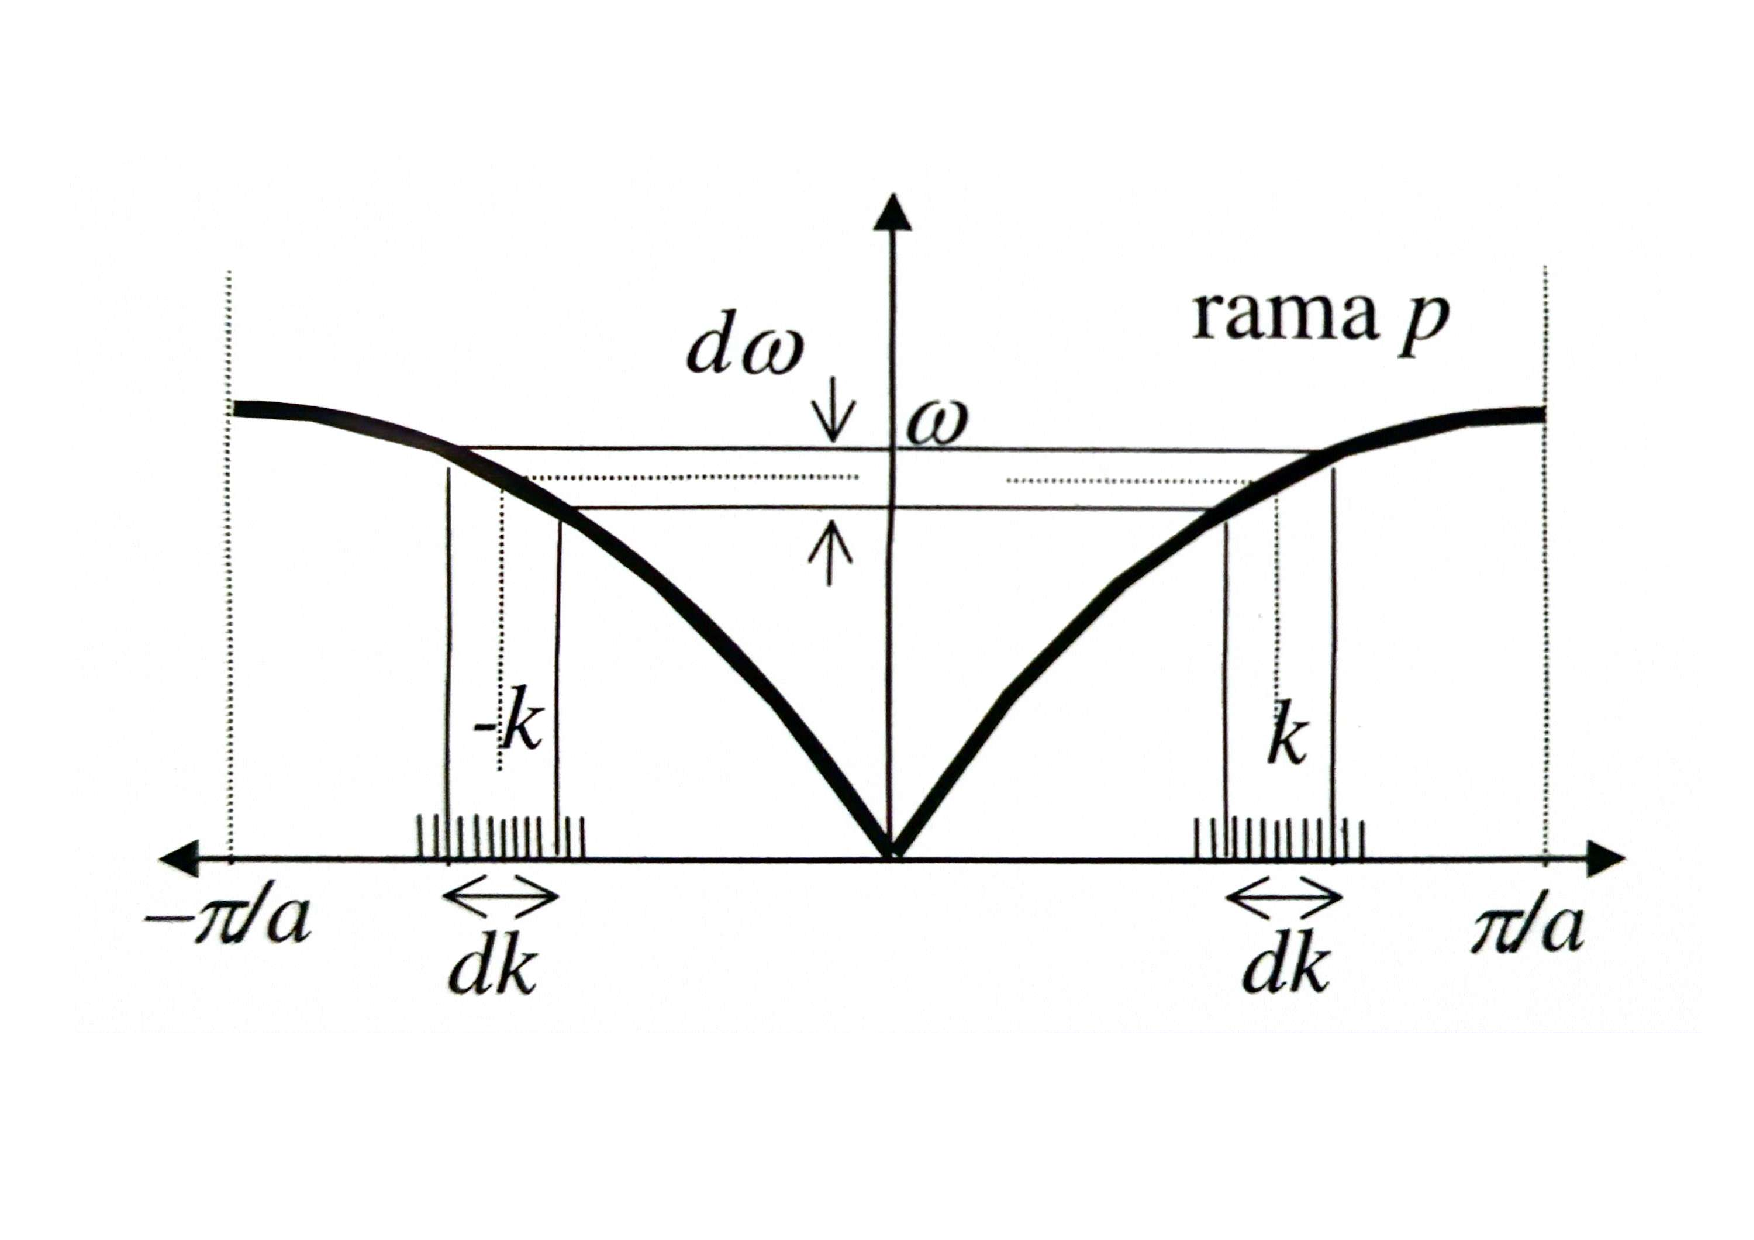
\includegraphics[scale=0.43]{Cuerpo/Ch_05/Fotos libro 1.pdf}
    \caption{Relación de dispersión para una cadena monoatómica. Equivalencia entre la densidad de modos en $k$ y en $\omega$.}
    \label{Fig:05-01}
\end{figure}    


\subsection{Cálculo de la densidad de modos}

Para el estudio de muchas propiedades cristalinas es importante conocer cómo se \textit{reparten} los modos posibles no en $\kn$ sino en frecuencia $\omega$. Se define así la \textit{densidad de modos} o \textit{estados} para la rama $p$, $D_p (\omega)$, como el número de modos por unidad de frecuencia con frecuencias en el intervalo $(\omega,\omega+\D \omega)$.

En una dimensión, si el cristal es de longitud $L=Na$, hay $N$ valores de $k$ en la $PZB$ ($-\pi/a < k\leq \pi/a$) de manera que, el intervalo $\delta k$ asociado a cada modo es $2 \pi / L$. El número de modos de una rama denotada por $p$ en el intervalo $\D \omega$ será, según se indica en la figura \ref{Fig:05-01}:

\begin{eqnarray*}
	D_p (\omega) \D \omega = \frac{2 \D k}{\delta k} = \frac{L}{\pi} \left| \parciales{k}{w}  \right| \D \omega = \frac{L}{\pi} \frac{\D \omega}{|\nabla_l \omega (k)|_p} \Rightarrow
\end{eqnarray*} 

\begin{eqnarray}
	D_p (\omega)  = \frac{L}{\pi} \frac{1}{|\nabla_ k \omega (k)|_p }
\end{eqnarray}
La generalización a dos y tres dimensiones es, respectivamente:

\begin{eqnarray}
	\text{2D}) \  D_p (\omega) &=& \int_{L_p (\omega)} \frac{S}{4\pi^2} \frac{\D L}{|\nabla_\kn \omega(\kn)|_p} \\ 
	\text{3D}) \  D_p (\omega) &=& \int_{S_p (\omega)} \frac{V}{8\pi^2} \frac{\D L}{|\nabla_\kn \omega(\kn)|_p} \label{Ec:05-01-04}
\end{eqnarray}
donde la integral se extiende sobre la línea (en 2D) o superficie (en 3D) del espacio $\kn$ con $\omega$. Finalmente, $D(\omega)=\sum_p Dp (\omega)$.
 
\subsection{Aproximación de Debye}

Esta aproximación consiste en sustituir todas las ramas de vibración por \textit{tres idénticas e isótropas} con relación de dispersión:

\begin{eqnarray}
	\omega = c k \quad (0<k<k_D)
\end{eqnarray}
siendo $c$ la velocidad del sonido en el cristal (para $k\rightarrow 0$) y $k_D$ el llamado \textbf{vector de onda de Debye}. Este se escoge de tal manera que el número total de modos sea el correcto ($3zN$). La figura \ref{Fig:05-02} ilustra como $k_D$ debe ser mayor que $k_{PZB}$ precisamente para que el número total de modos sea el adecuado. Según esta definición

\begin{eqnarray}
	3zN = 3 \times \frac{\frac{4}{3} \pi k^3_D}{\frac{8 \pi^3}{V}} \Rightarrow k_D^3 = 6 \pi^2 n
\end{eqnarray}
siendo $n=zN/V$ la densidad numérica de átomos. 

En esta aproximación las superficies de $\omega$ constante son esferas (la figura \ref{Fig:05-03} muestra la sección para $k_z$ de una superficie $\omega=\cte.$) La densidad de modos viene dada por $D_D(\omega) \D \omega = 3 \times 4 \pi k^2 \D k / (8\pi3 /V)$, que al utilizar (\ref{Ec:05-01-04}) permite despejar 

\begin{eqnarray}
	D_D (\omega) = \frac{3V}{2\pi^2} \frac{\omega^2}{c^3} \tquad (0<\omega<\omega_D)
\end{eqnarray}
La frecuencia máxima $\omega_D=ck_D$ se denomina \textbf{frecuencia de Debye}.

\begin{figure}[h!] \centering
    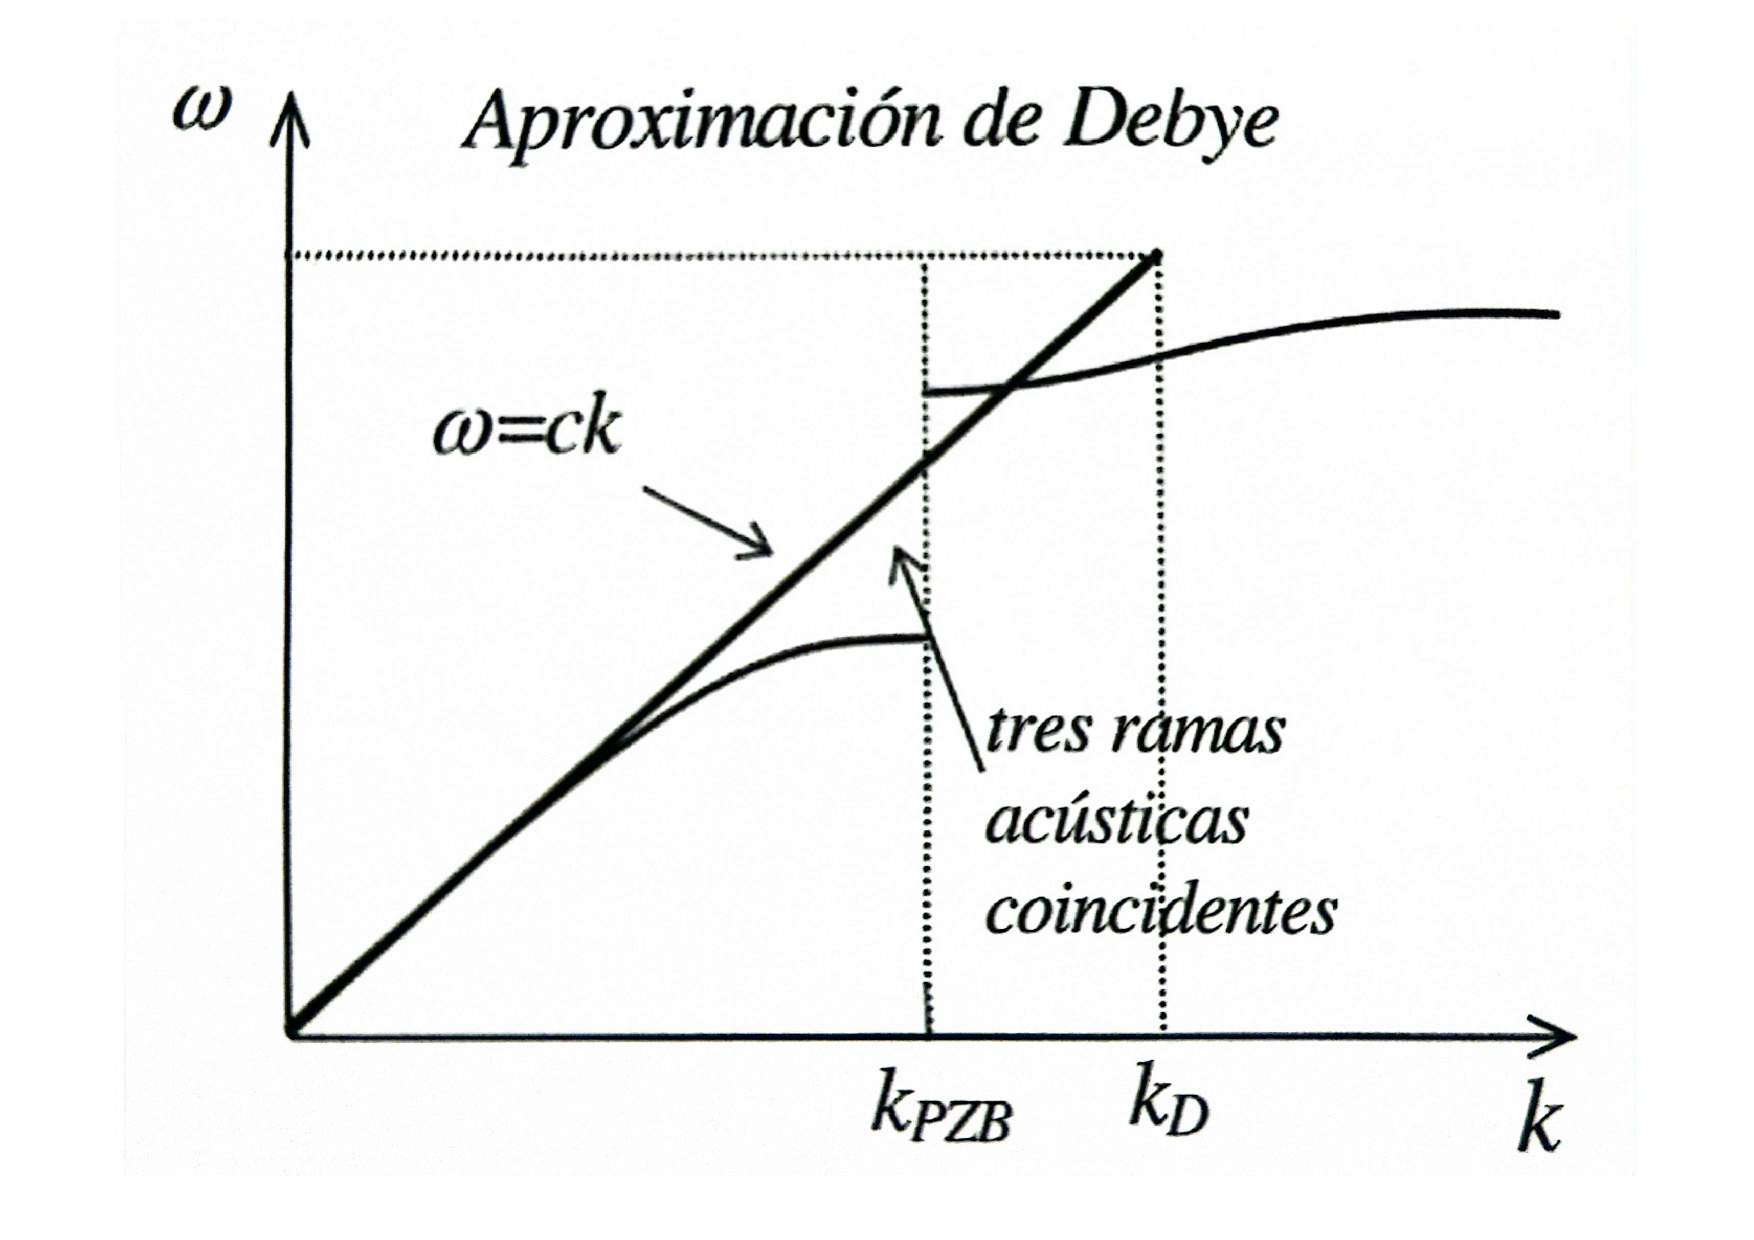
\includegraphics[scale=0.43]{Cuerpo/Ch_05/Fotos libro 2.pdf}
    \caption{Representación de la aproximación de Debye. Todas las ramas se sustituyen por tres acústicas degeneradas.}
    \label{Fig:05-02}
\end{figure}    


\section{Capacidad térmica reticular}

\subsection{Estadística de fonones}

\begin{figure}[h!] \centering
    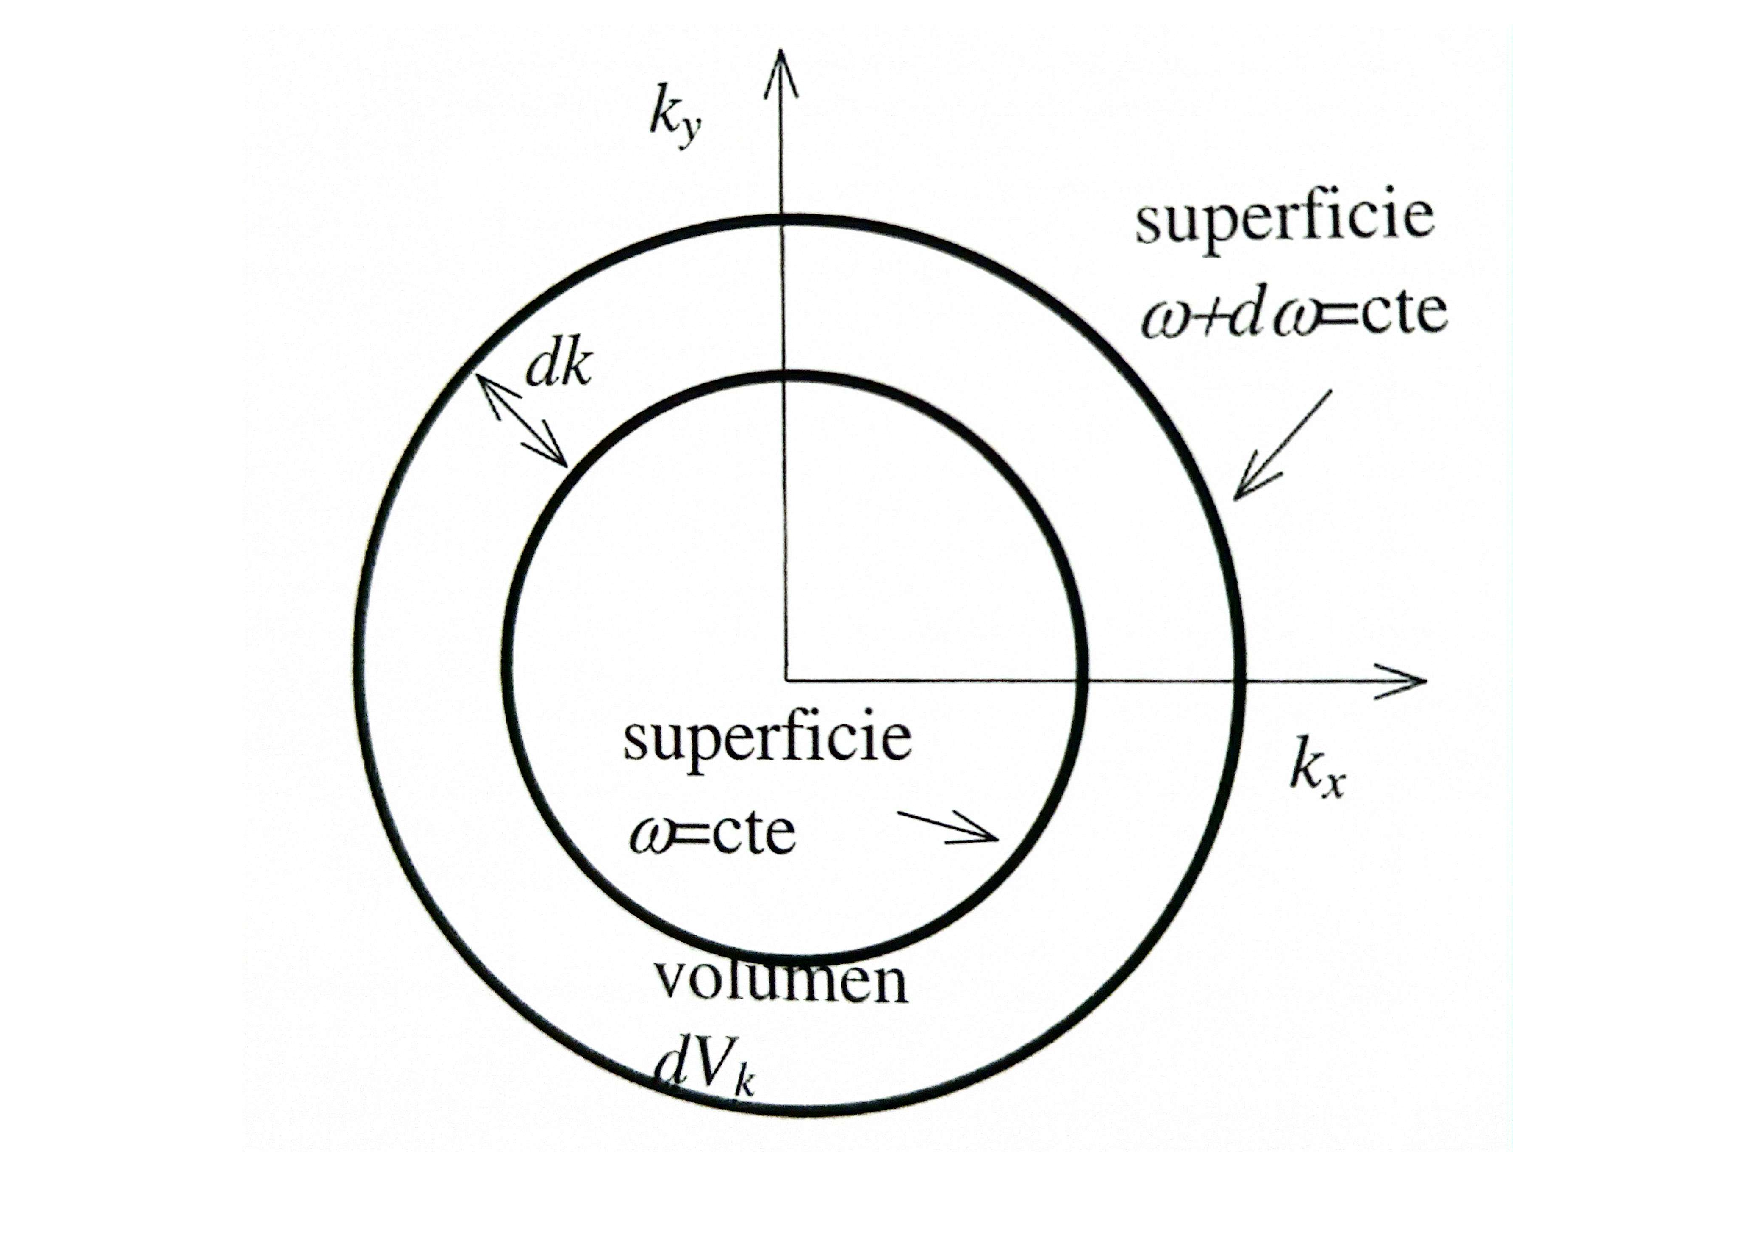
\includegraphics[scale=0.5]{Cuerpo/Ch_05/Fotos libro 3.pdf}
    \caption{Sección de una superficie de frecuencia constante en la aproximación de Debye.}
    \label{Fig:05-03}
\end{figure}    


\subsection{Cálculo de la capacidad térmica}

\begin{figure}[h!] \centering
    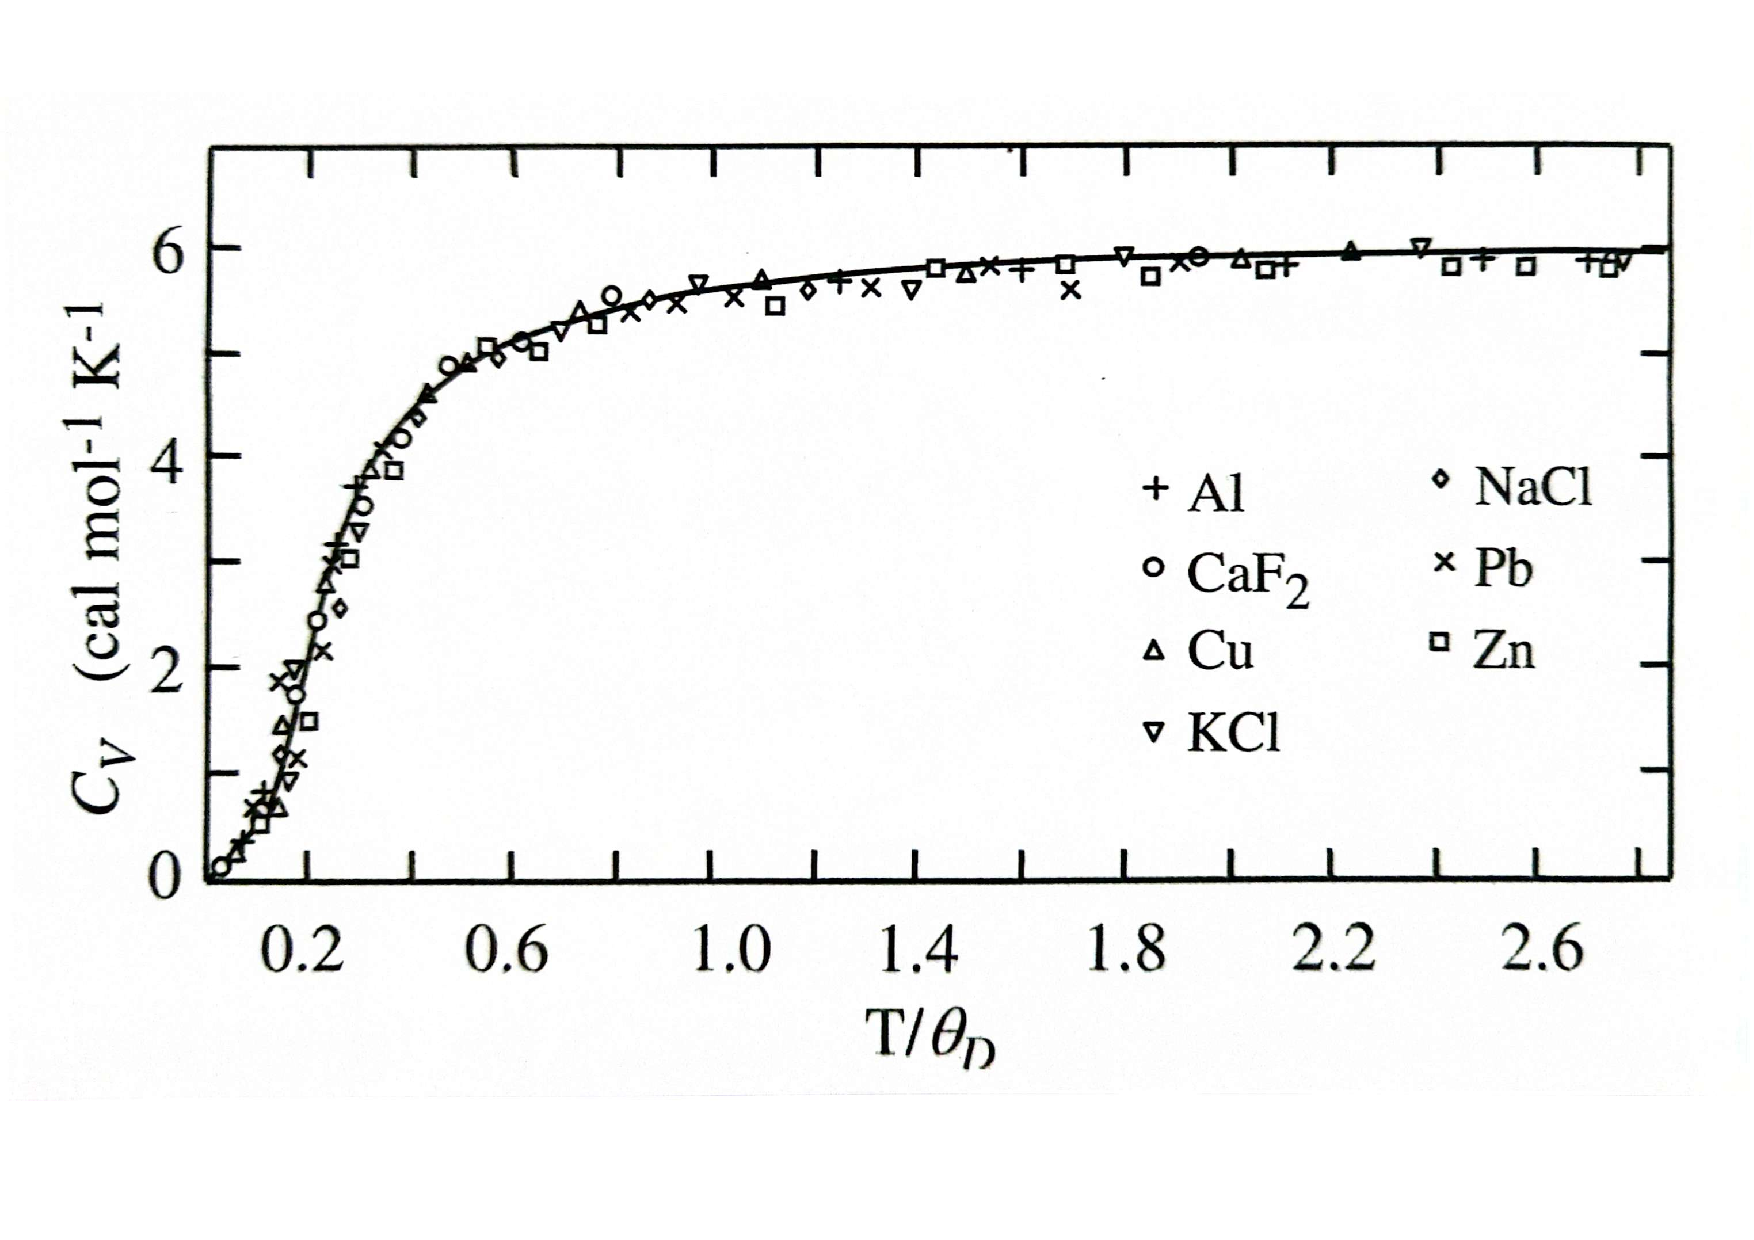
\includegraphics[scale=0.5]{Cuerpo/Ch_05/Fotos libro 4.pdf}
    \caption{Capacidad térmica por mol frente $T/\theta_D$ para diversos tipos de cristales.}
    \label{Fig:05-04}
\end{figure}    



\section{Efectos anarmónicos}

\subsection{Dilatación térmica}

\begin{figure}[h!] \centering
    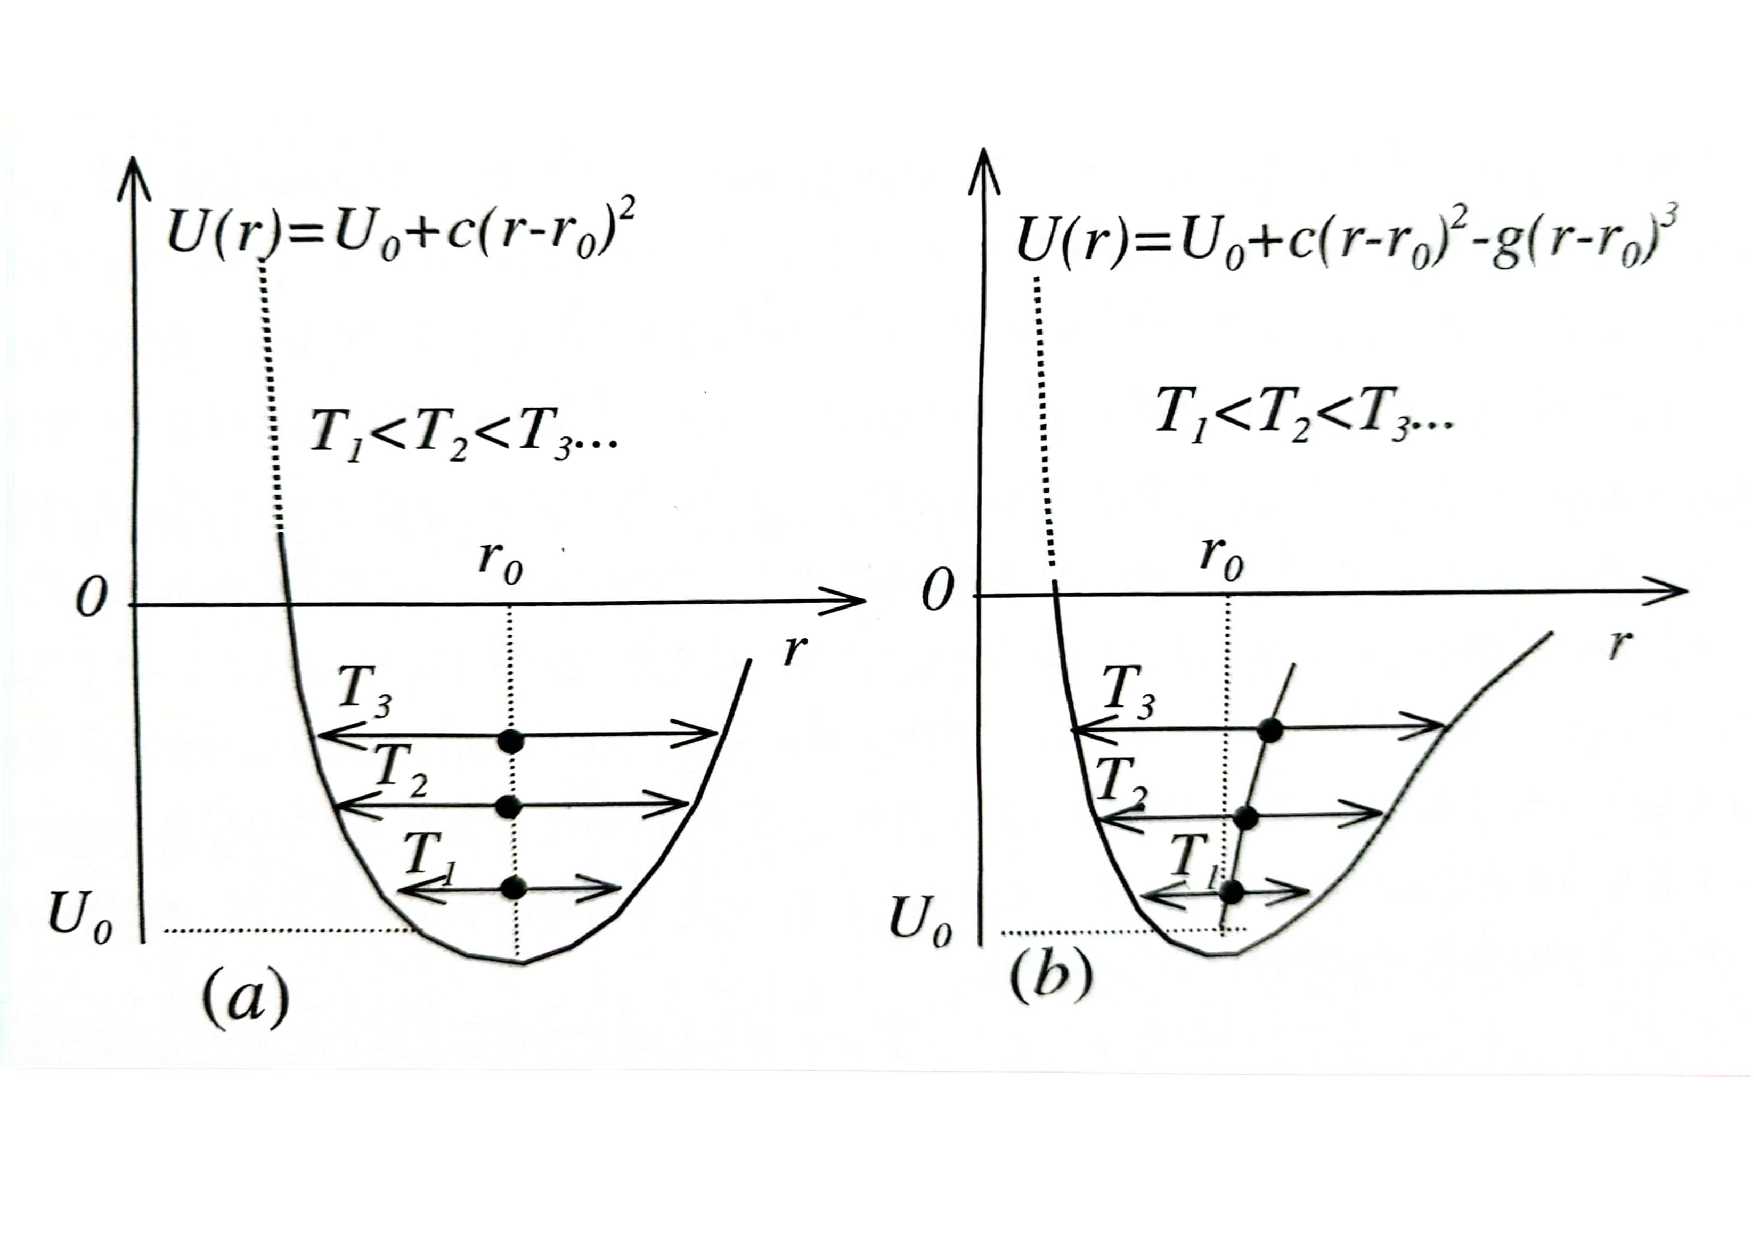
\includegraphics[scale=0.5]{Cuerpo/Ch_05/Fotos libro 5.pdf}
    \caption{Potencial por par de átomos según la aproximación armónica (a) y según la aproximación anarmónica (b) que permite explicar de los cristales cuando se calientan.}
    \label{Fig:05-05}
\end{figure}    


\subsection{Conductividad térmica}

\begin{figure}[h!] \centering
    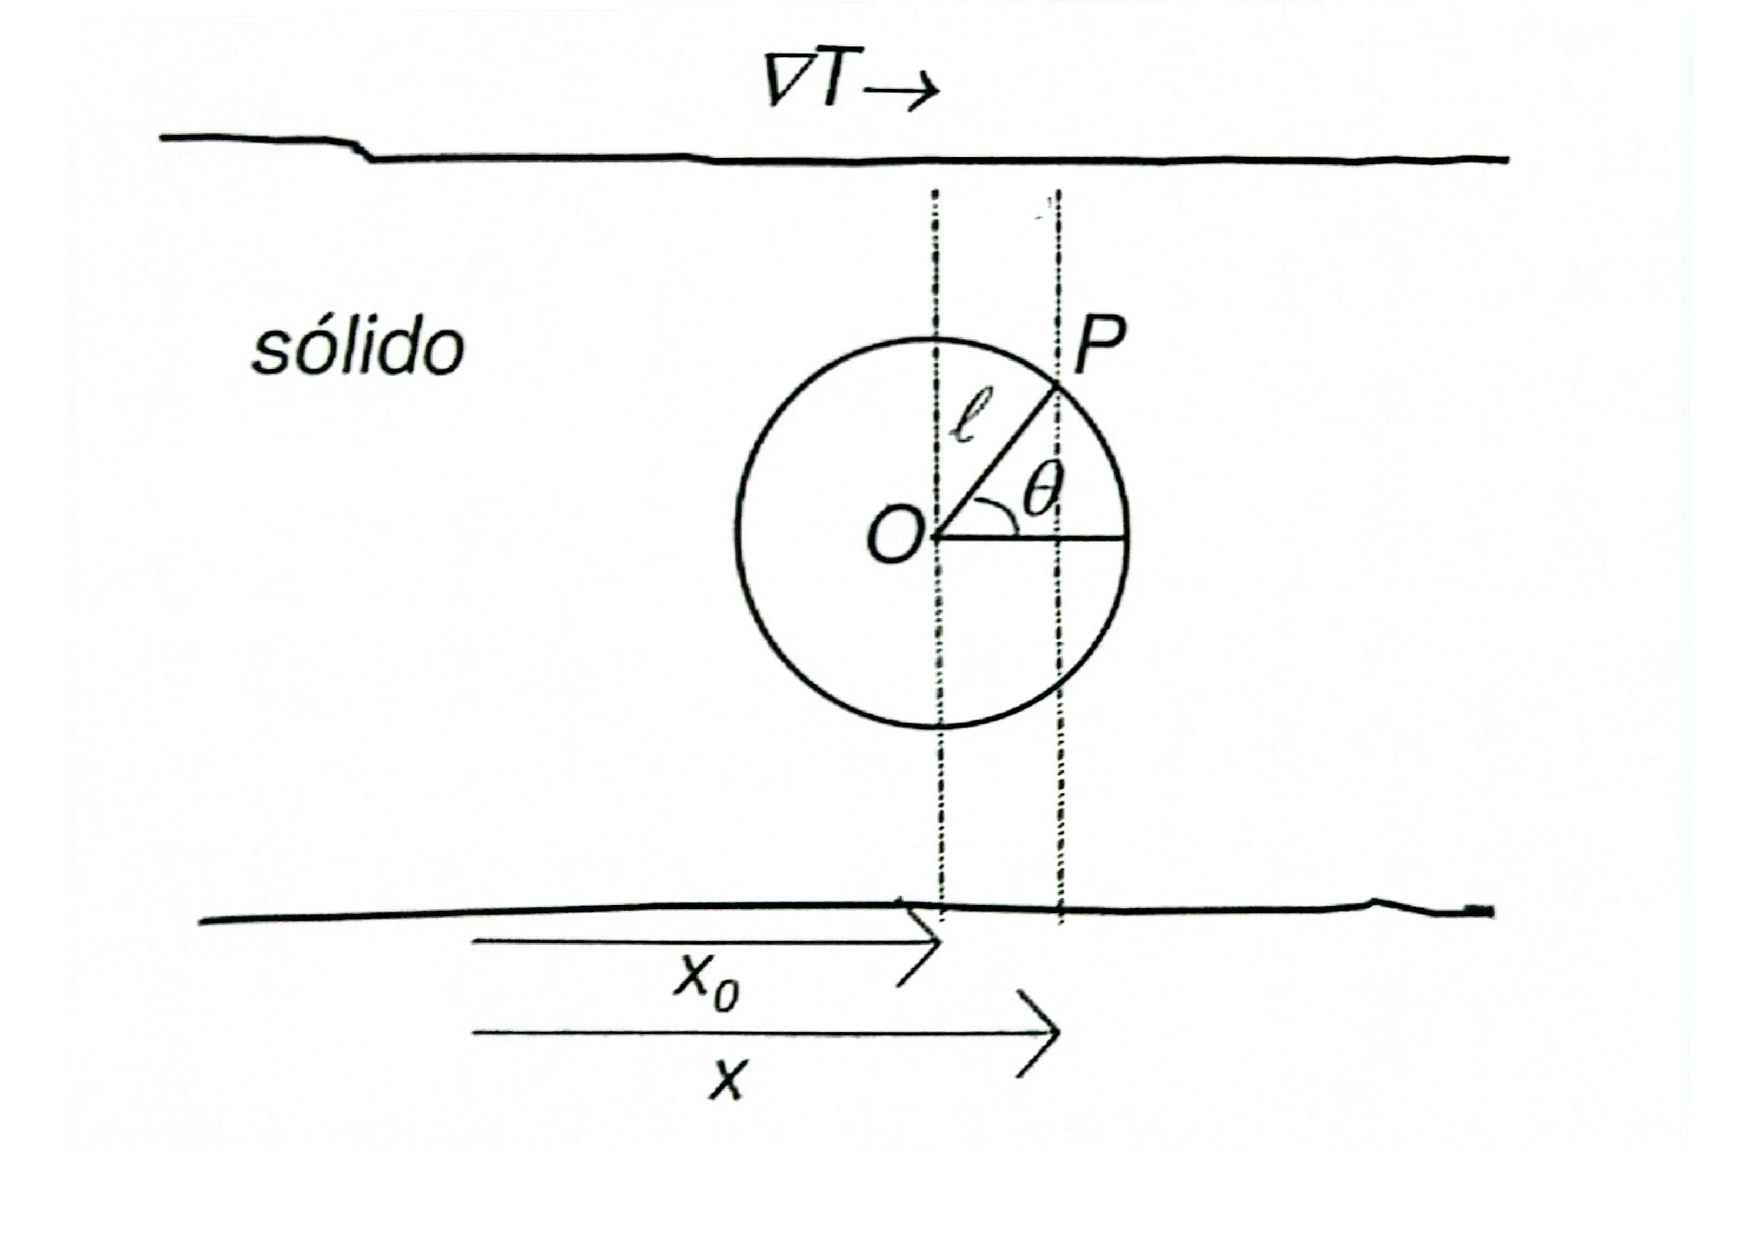
\includegraphics[scale=0.5]{Cuerpo/Ch_05/Fotos libro 6.pdf}
    \caption{Transporte de calor mediante fonones en presencia de un gradiente uniforme de temperatura. La corriente térmica en $O$ se debe a los fonones que, en media, han sufrido la última colisión en un punto $P$ a distancia $l=c\tau$.}
    \label{Fig:05-06}
\end{figure}    
\begin{figure}[h!] \centering
    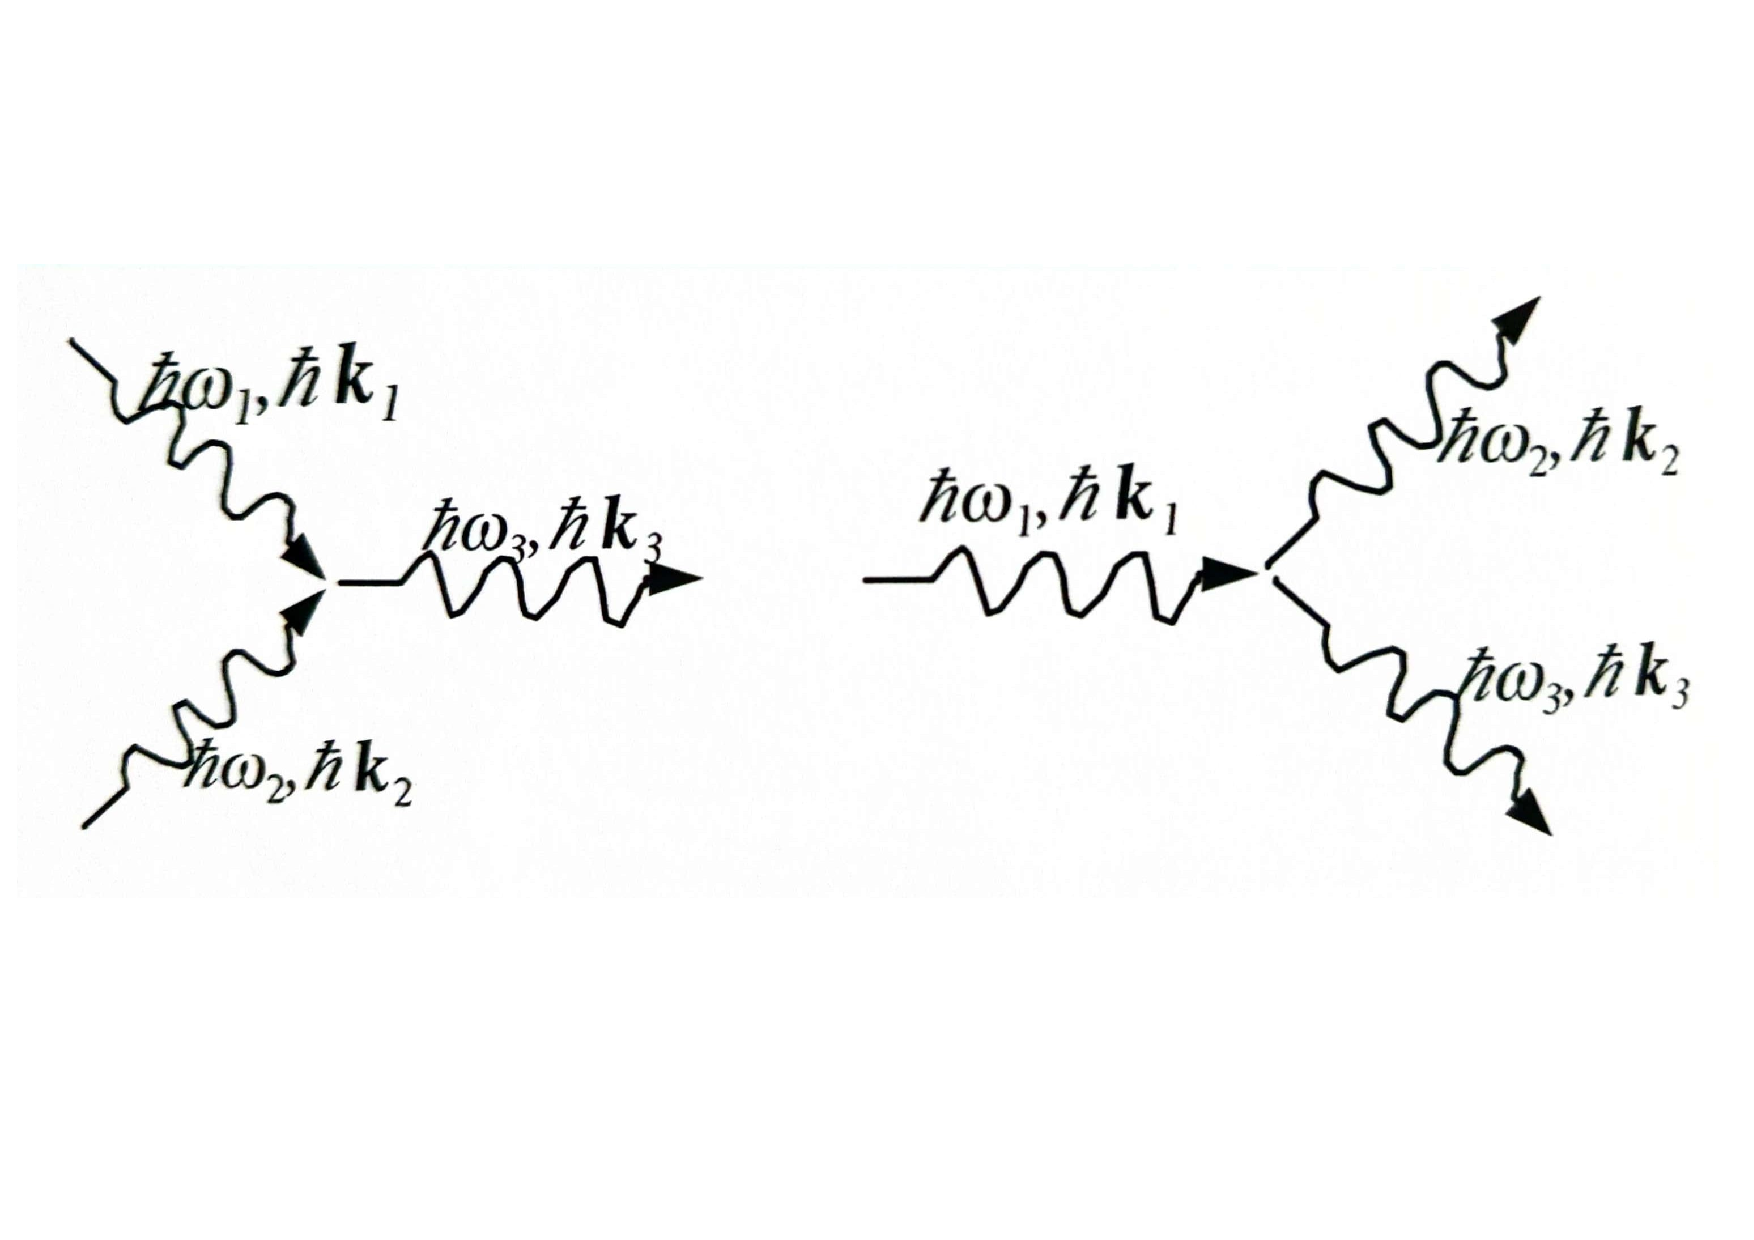
\includegraphics[scale=0.5]{Cuerpo/Ch_05/Fotos libro 7.pdf}
    \caption{Procesos de interacción entre fonones debidos a los términos (\textit{cúbicos}) anarmónicos del potencial de interacción entre átomos. Izquierda: Dos fonones interaccionan dando lugar a un tercer fonón. Derecha: Un fonón \textit{se rompe} en dos.}
    \label{Fig:05-07}
\end{figure}    
\begin{figure}[h!] \centering
    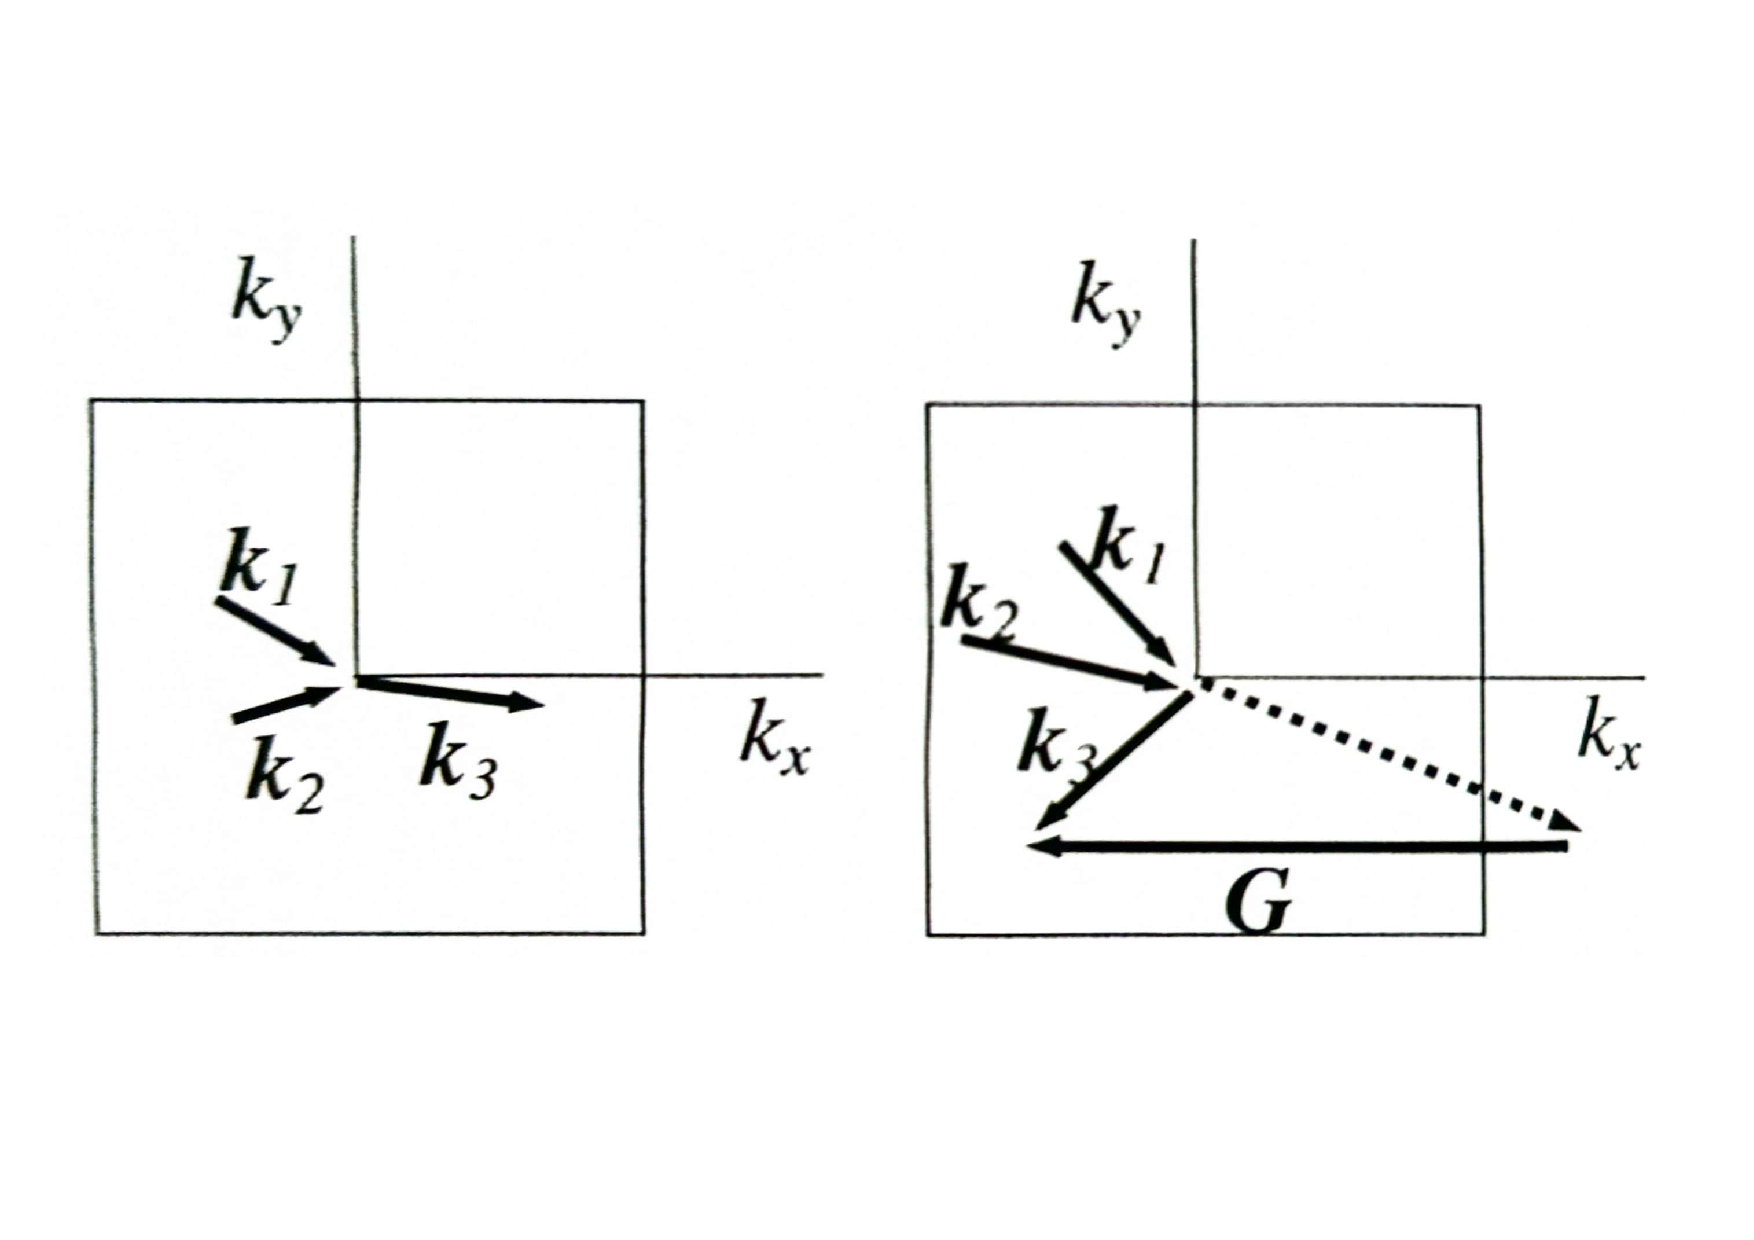
\includegraphics[scale=0.5]{Cuerpo/Ch_05/Fotos libro 8.pdf}
    \caption{Izquierda: Proceso $N$ que no degrada el transporte de energía térmica. Derecha: Proceso $U$ que degrada fuertemente el transporte de calor.}
    \label{Fig:05-08}
\end{figure}    
\begin{figure}[h!] \centering
    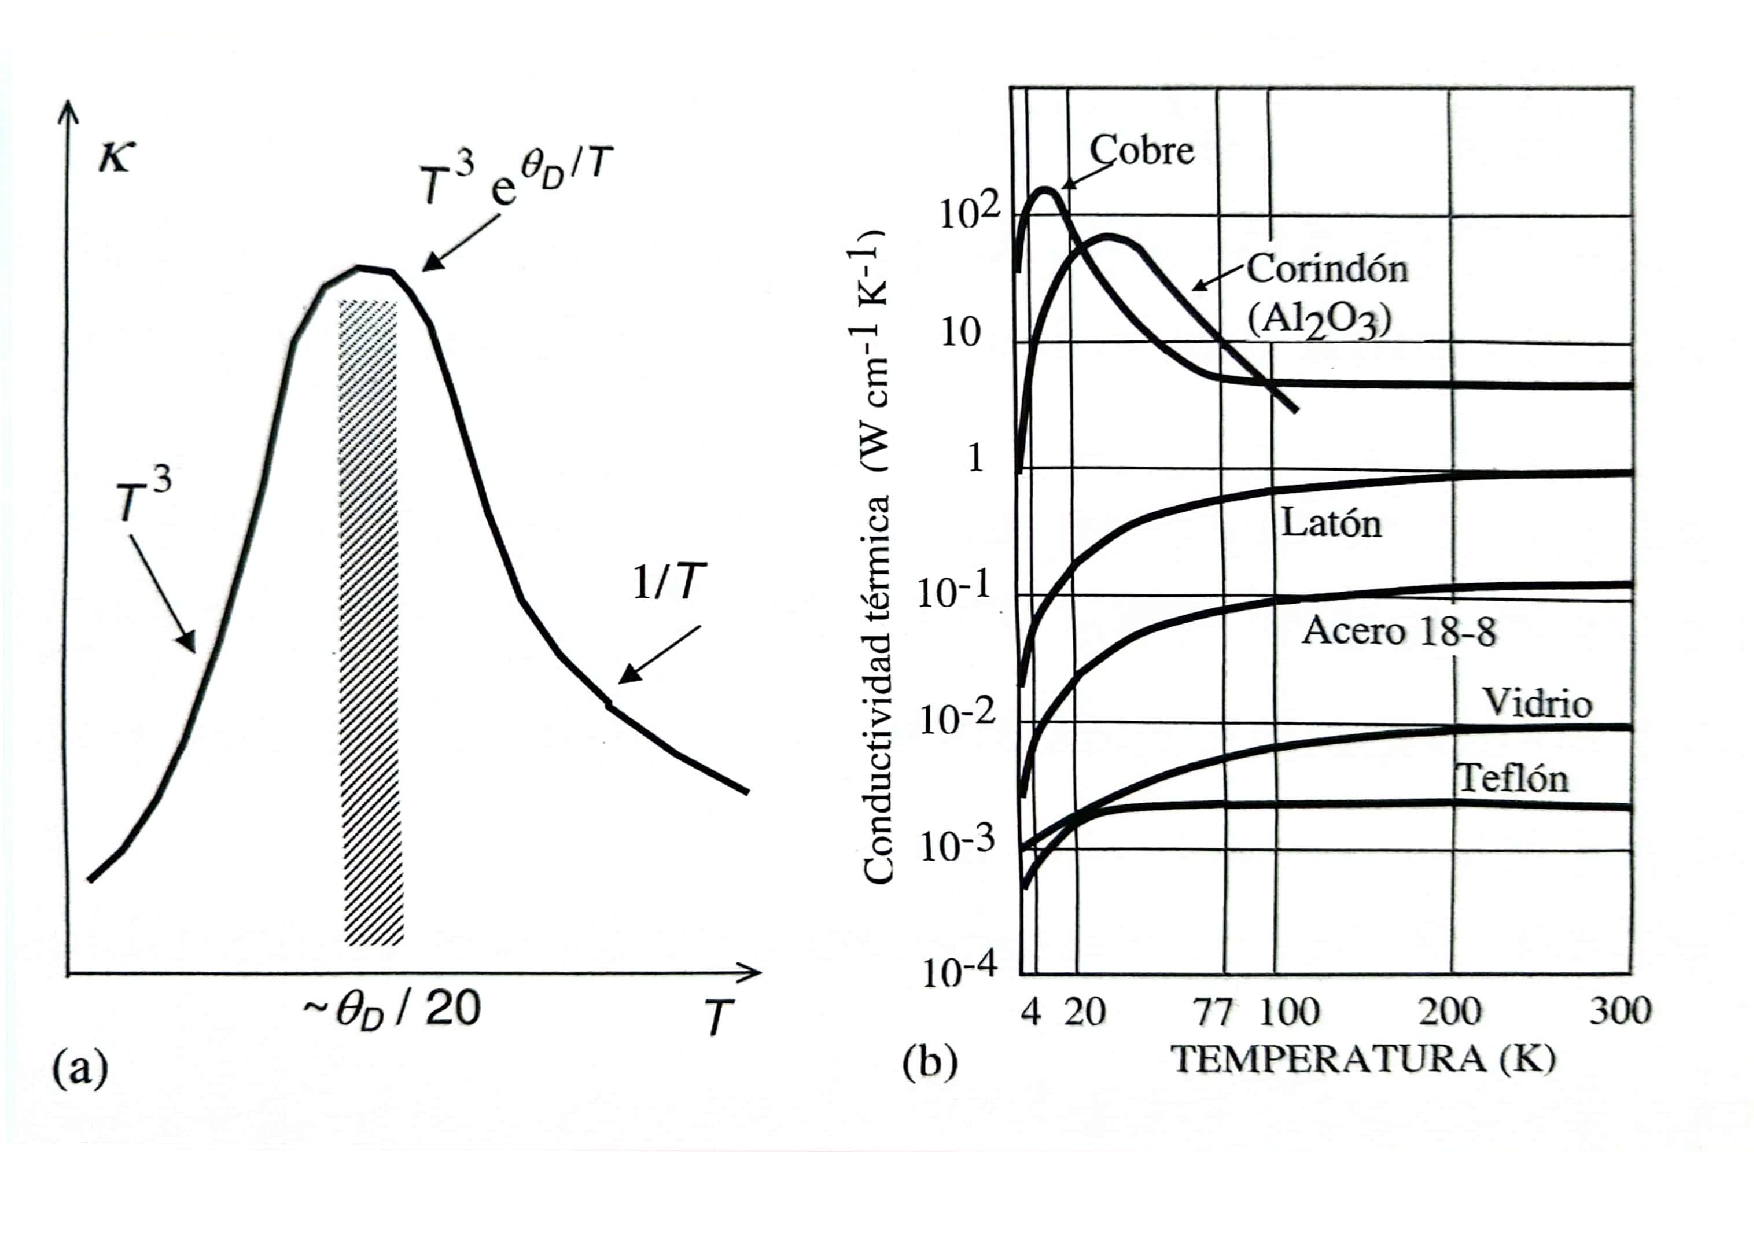
\includegraphics[scale=0.5]{Cuerpo/Ch_05/Fotos libro 9.pdf}
    \caption{(a) Dependencia genérica de la conductividad térmica de los cristales con la temperatura. (b) Conductividad térmica frente a la temperatura para diversos tipos de sólidos.}
    \label{Fig:05-09}
\end{figure}    

